\documentclass[border=10pt]{standalone}

\usepackage{tikz}
\usepackage{tikzsymbols}
\usetikzlibrary{calc,patterns,shapes.geometric}

\def\centerarc[#1](#2)(#3:#4:#5){\draw[#1] ($(#2)+({#5*cos(#3)},{#5*sin(#3)})$) arc (#3:#4:#5);}

\begin{document}
	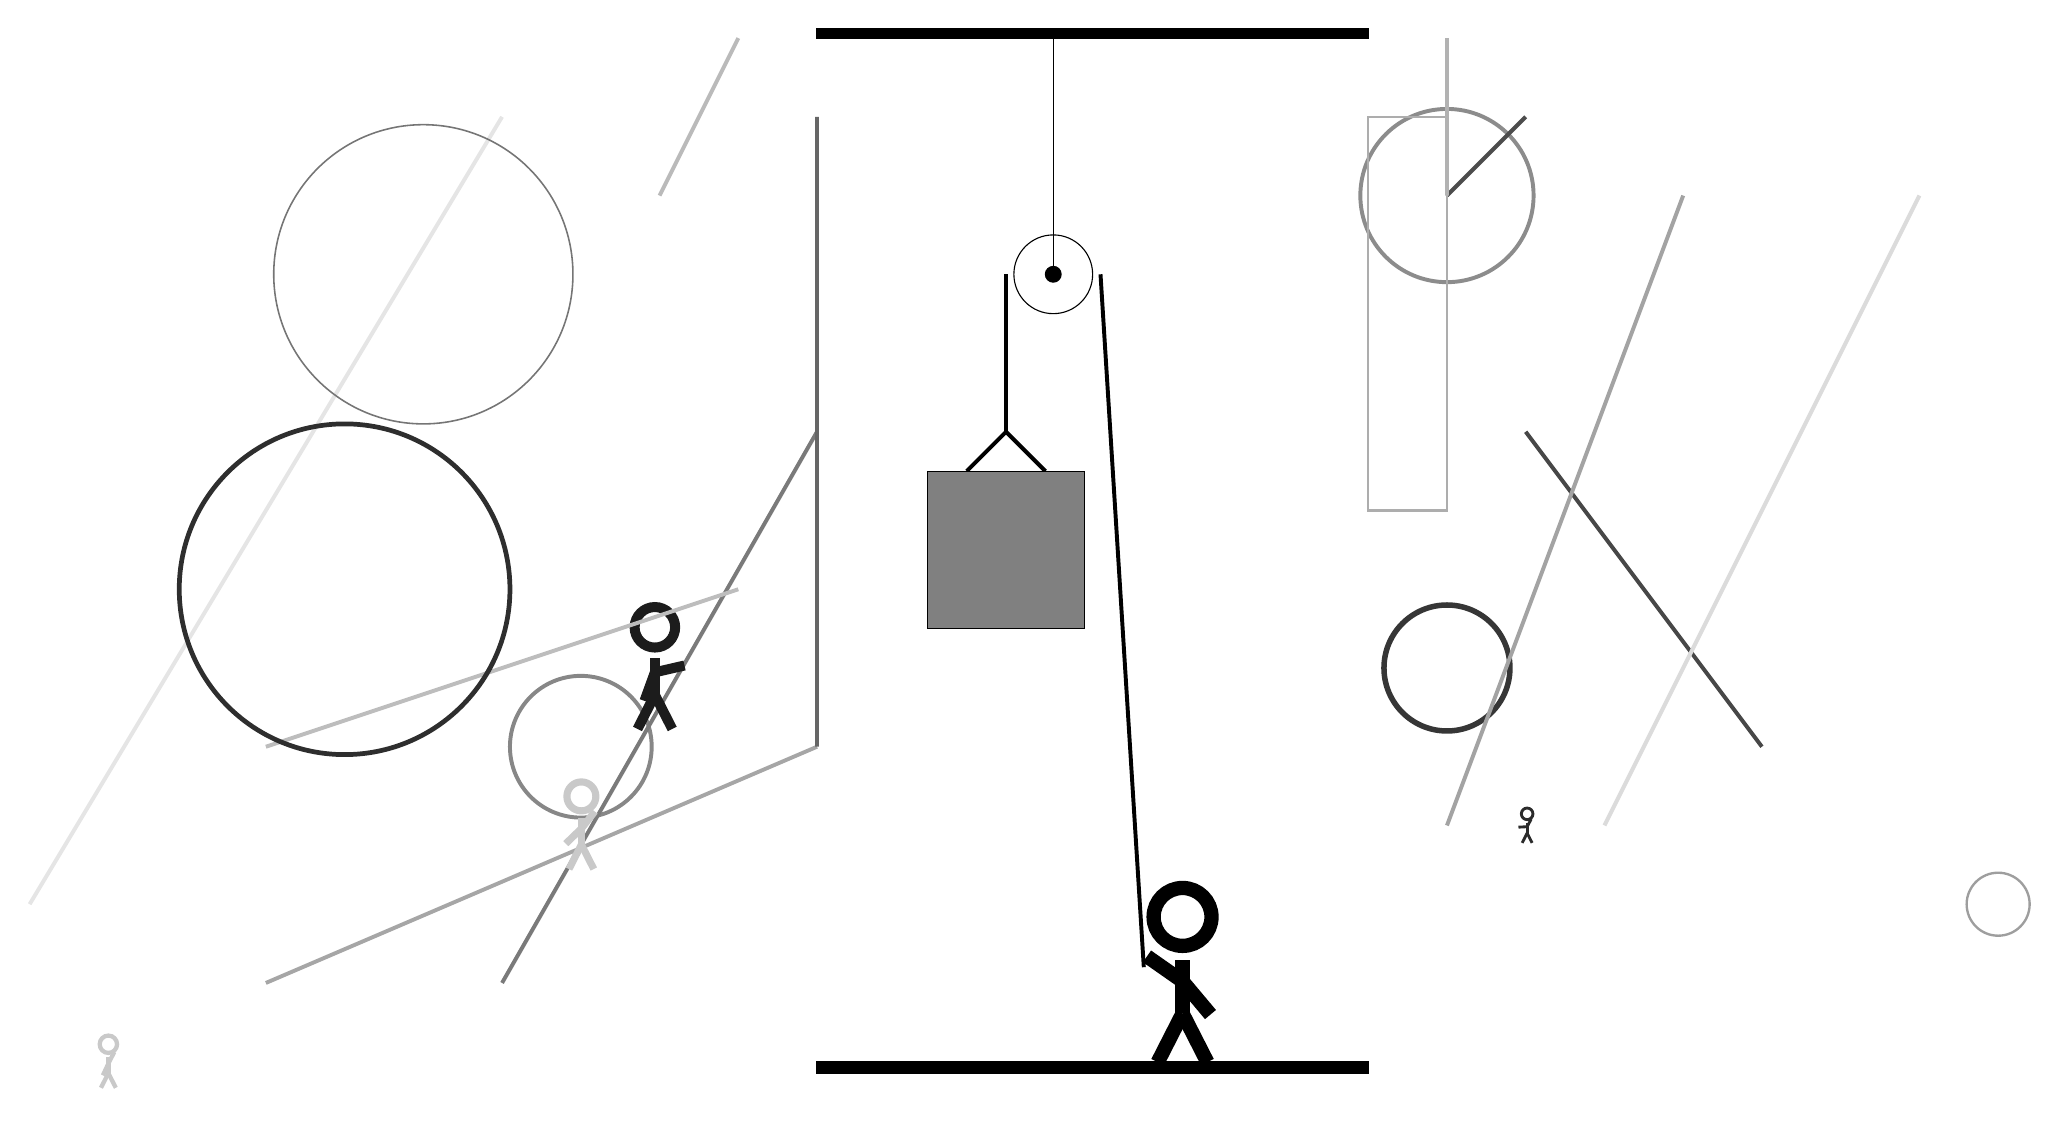
\begin{tikzpicture}
		%%%%% START %%%%%
		
		\draw[fill=black] (-2, 10) rectangle (5, 10.125);
		
		\draw (1, 7) circle (0.5);
		\draw[fill=black] (1, 7) circle (0.1);
		\draw (1, 10) -- (1, 7);
		
		\draw[line width=0.5mm] (-0.1, 4.5) -- (0.4, 5.0) -- (0.9, 4.5);
		\draw[fill=black!50] (-0.6, 4.5) rectangle (1.4, 2.5);
		
		\draw[line width=0.5mm] (0.4, 7) -- (0.4, 5.0);
		\centerarc[line width=0.5mm](1, 7)(0:180:0.6);
		\draw[line width=0.5mm](1.6, 7) -- (2.15, -1.8);
		
		\node at (2.6, -1.9) {\Strichmaxerl[10][-35][-50]};
		
		\draw[line width=0.5mm, color=black!35](-2, 1) -- (-9, -2);
		
		\draw [line width=0.5mm, color=black!47](-5, 1) circle (0.9);
		\draw [line width=0.5mm, color=black!45](6, 8) circle (1.1);
		\draw[line width=0.5mm, color=black!10](-6, 9) -- (-12, -1);
		\draw[line width=0.5mm, color=black!52](-6, -2) -- (-2, 5);
		\node[line width=0.4mm, color=black!83] at (7, 0) {\Strichmaxerl[2][3][62]};
		\node[line width=0.5mm, color=black!89] at (-4, 2) {\Strichmaxerl[7][70][13]};
		\draw [line width=0.2mm, color=black!54](-7, 7) circle (1.9);
		\draw[line width=0.5mm, color=black!26](-3, 3) -- (-9, 1);
		
		\draw [line width=0.6mm, color=black!82](-8, 3) circle (2.1);
		\node[line width=0.2mm, color=black!21] at (-5, 0) {\Strichmaxerl[5][44][52]};
		\draw[line width=0.5mm, color=black!72](7, 5) -- (10, 1);
		\draw[line width=0.5mm, color=black!14](8, 0) -- (12, 8);
		\draw[line width=0.5mm, color=black!70](7, 9) -- (6, 8);
		\draw[line width=0.3mm, color=black!32] (5, 4) rectangle (6, 9);
		\draw[line width=0.6mm, color=black!60] (-2, 9) rectangle (-2, 1);
		\draw [line width=0.3mm, color=black!38](13, -1) circle (0.4);
		\draw[line width=0.5mm, color=black!30] (6, 10) rectangle (6, 8);
		\draw [line width=0.7mm, color=black!79](6, 2) circle (0.8);
		
		\draw[line width=0.5mm, color=black!27](-4, 8) -- (-3, 10);
		\node[line width=0.4mm, color=black!21] at (-11, -3) {\Strichmaxerl[3][65][63]};
		
		\draw[line width=0.5mm, color=black!36](6, 0) -- (9, 8);
		
		\draw[fill=black] (-2, -3) rectangle (5, -3.15);
		
		%%%%% END %%%%%
	\end{tikzpicture}
\end{document}